%! Author = Omar Iskandarani
%! Title = The Vortex Æther Model: A Unified Topological Field Theory of Mass, Gravity, and Time
%! Date = ...
%! Affiliation = Independent Researcher, Groningen, The Netherlands
%! License = CC-BY 4.0
%! ORCID = 0009-0006-1686-3961
%! DOI = ..

\newcommand{\paperdoi}{...}
\documentclass[12pt,aps,prd,onecolumn,nofootinbib,superscriptaddress]{revtex4-2}

% ==================== Packages ====================
\usepackage[utf8]{inputenc}
\usepackage[T1]{fontenc}
\usepackage{lmodern}
\usepackage{amsmath,amssymb,amsfonts}
\usepackage{graphicx}
\usepackage{hyperref}
\usepackage{doi}
\usepackage{physics}
\usepackage{mathtools}
\usepackage{tikz}
\usetikzlibrary{knots,intersections,decorations.pathreplacing}
\usetikzlibrary{3d, calc, arrows.meta, positioning}
\usepackage{pgfmath}
\usetikzlibrary{decorations.pathmorphing}
\usepackage{pgfplots}
\pgfplotsset{compat=1.18} % or version you have
\usepackage{bm}          % bold math
\usepackage{titlesec}    % section formatting (optional)
\usepackage{float}       % [H] float placement
\newcommand{\knotgif}[1]{\includegraphics[height=1.2em]{images/#1.gif}}
% ==================== Metadata ====================
\begin{document}

\title{The Vortex Æther Model: \\[1ex]
        \large A Unified Topological Field Theory of Mass, Gravity, and Time}

\author{Omar Iskandarani}
\email{info@omariskandarani.com}
\affiliation{Independent Researcher, Groningen, The Netherlands}
\thanks{ORCID: \href{https://orcid.org/0009-0006-1686-3961}{0009-0006-1686-3961}}
\thanks{DOI: \href{https://doi.org/\paperdoi}{\paperdoi}}
\thanks{License: CC-BY 4.0 International}
    
\date{\today}

% ==================== Abstract ====================
\begin{abstract}
            We present the Vortex Æther Model (VAM), a unified physical framework in which mass, gravity, and proper time emerge from topologically structured vorticity within a compressible, inviscid æther. In contrast to curvature-based relativity and Higgs-based mass generation, VAM describes particles as knotted vortex excitations, and gravity as a swirl-induced time deviation field. The theory reproduces classical phenomena such as gravitational redshift, time dilation, and frame-dragging through fluid-dynamic energetics, and calculates particle masses and physical constants from first principles. The Standard Model gauge groups SU(3), SU(2), and U(1) arise naturally from vortex topology and swirl symmetry, while canonical quantization defines a Fock-like Hilbert space over knot eigenstates. We develop a full path-integral formulation over topological sectors of the æther manifold, enabling quantum transitions, knot fusion, and helicity exchange interactions. Benchmarking against general relativity and experimental tests of gravitational time deviation support the model’s viability. VAM offers a physically grounded, falsifiable, and derivational alternative to conventional quantum gravity and field theory models.
\end{abstract}
\maketitle

        \begin{figure}[H]
            \centering
            \footnotesize
            \scalebox{0.75}{
                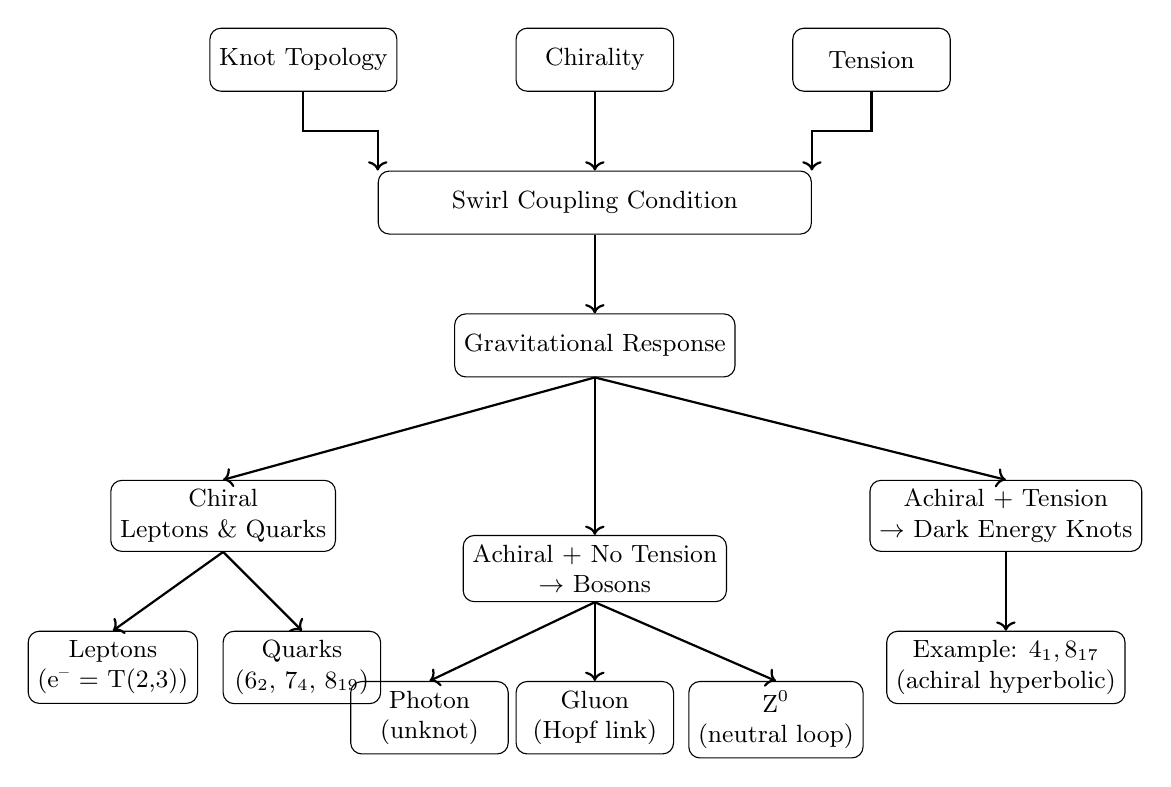
\begin{tikzpicture}[
                  box/.style = {draw, rounded corners, minimum width=2.0cm, minimum height=0.8cm, font=\small, align=center},
                  arrow/.style = {->, thick},   node distance=1.0cm and 1.5cm
                ]
                    % Inputs
                    \node[box] (topology) {Knot Topology};
                    \node[box, right=of topology] (chirality) {Chirality};
                    \node[box, right=of chirality] (tension) {Tension};

                    % Swirl coupling
                    \node[box, below=of chirality, minimum width=5.5cm] (coupling) {Swirl Coupling Condition};

                    % Gravitational response
                    \node[box, below=of coupling] (grav) {Gravitational Response};

                    % Gravitational classes
                    \node[box, below left=1.3cm and 1.5cm of grav] (matter) {Chiral\\Leptons \& Quarks};
                    \node[box, below=2cm of grav] (boson) {Achiral + No Tension\\\(\rightarrow\) Bosons};
                    \node[box, below right=1.3cm and 1.7cm of grav] (dark) {Achiral + Tension\\\(\rightarrow\) Dark Energy Knots};

                    % Subclasses
                    \node[box, below=of matter, xshift=-1.4cm] (leptons) {Leptons\\(e\textsuperscript{--} = T(2,3))};
                    \node[box, below=of matter, xshift=+1.0cm] (quarks) {Quarks\\(6\textsubscript{2}, 7\textsubscript{4}, 8\textsubscript{19})};

                    \node[box, below=of boson, xshift=-2.1cm] (photon) {Photon\\(unknot)};
                    \node[box, below=of boson] (gluon) {Gluon\\(Hopf link)};
                    \node[box, below=of boson, xshift=+2.3cm] (zboson) {Z\textsuperscript{0}\\(neutral loop)};

                    \node[box, below=of dark] (darkex) {Example: \(4_{1}, 8_{17}\)\\ (achiral hyperbolic)};

                    % Arrows to coupling
                    \draw[arrow] (topology.south) -- ++(0,-0.5) -| (coupling.north west);
                    \draw[arrow] (chirality.south) -- (coupling.north);
                    \draw[arrow] (tension.south) -- ++(0,-0.5) -| (coupling.north east);

                    % Arrows down flow
                    \draw[arrow] (coupling.south) -- (grav.north);
                    \draw[arrow] (grav.south) -- (matter.north);
                    \draw[arrow] (grav.south) -- (boson.north);
                    \draw[arrow] (grav.south) -- (dark.north);

                    % Particle branches
                    \draw[arrow] (matter.south) -- (leptons.north);
                    \draw[arrow] (matter.south) -- (quarks.north);

                    \draw[arrow] (boson.south) -- (photon.north);
                    \draw[arrow] (boson.south) -- (gluon.north);
                    \draw[arrow] (boson.south) -- (zboson.north);

                    \draw[arrow] (dark.south) -- (darkex.north);
                \end{tikzpicture}
            }
            \caption{Knot Classification by Swirl Coupling.
                The flowchart visualizes how knot topology, chirality, and curvature tension determine gravitational behavior, and how this leads to specific particle subclasses:
                    \\ \textbf{Chiral knots} align with swirl fields and form matter: \textbf{leptons} (torus knots) and \textbf{quarks} (hyperbolic knots).
                    \\ \textbf{Achiral, tensionless} structures like unknots and Hopf links are \textbf{bosons}, passively guided by swirl tubes.
                    \\ \textbf{Achiral knots with tension} are expelled, forming \textbf{dark energy} candidates.
            }\label{fig:knot-classification}
        \end{figure}


% ==================== Table of Contents (optional) ====================
\tableofcontents
\vspace{1em}
\hrule
\vspace{1em}
\newpage
% ==================== Main Body ====================
\section{knot not knots}
test versions of inline knot images:\\
 \( 0_1 \):~\includegraphics[height=1.2em]{images/0_1} \( 2_1 \):~\includegraphics[height=1.2em]{images/hopf}\\
 \( 2_1 \):~\includegraphics[height=1.2em]{images/ahopf}\\
 \( 2_1 \):~\includegraphics[height=1.2em]{images/solomon}\\
 \( 2_1 \):~\includegraphics[height=1.2em]{images/asolomon}\\
 \( 2_1 \):~\includegraphics[height=1.2em]{images/borromean}\\
 \( 2_1 \):~\includegraphics[height=1.2em]{images/aborromean}\\
 \( T(3,2) \):~\includegraphics[height=1.2em]{images/3_1}\\
 \( T(2,3) \):~\includegraphics[height=1.2em]{images/a3_1}\\
 \( 6_2 \):~\includegraphics[height=1.2em]{images/6_2}\\
 \( 7_4 \):~\includegraphics[height=1.2em]{images/7_4}\\
 \( 4_1 \):~\includegraphics[height=1.2em]{images/4_1}
\begin{tikzpicture}[scale=0.1,  line width=0.4pt]
  \def\nsamples{60}
  \foreach \i in {1,...,\nsamples} {
      \pgfmathsetmacro\tprev{(\i - 1) * 2 * pi / \nsamples}
      \pgfmathsetmacro\tcurr{\i * 2 * pi / \nsamples}
      \pgfmathsetmacro\xprev{(2 + cos(2 * \tprev r)) * cos(3 * \tprev r)}
      \pgfmathsetmacro\yprev{(2 + cos(2 * \tprev r)) * sin(3 * \tprev r)}
      \pgfmathsetmacro\xcurr{(2 + cos(2 * \tcurr r)) * cos(3 * \tcurr r)}
      \pgfmathsetmacro\ycurr{(2 + cos(2 * \tcurr r)) * sin(3 * \tcurr r)}
      \draw[black, --] (\xprev,\yprev) -- (\xcurr,\ycurr);
  }
\end{tikzpicture}\\
 \( 5_1 \):~\includegraphics[height=1.2em]{images/5_1}\\
 \( 5_2 \):~\includegraphics[height=1.2em]{images/5_2}\\
 \( 7_2 \):~\includegraphics[height=1.2em]{images/7_2}\\





\section*{Introduction}
We compare the Vortex Æther Model (VAM) – a fluid-dynamic analogue of gravity – against General Relativity (GR) (and Special Relativity where applicable) across classical and modern tests. Five representative objects (electron, proton, Earth, Sun, neutron star) span quantum to astrophysical scales. For each key relativistic phenomenon, we present theoretical predictions from GR and VAM, compare to observed values, and note agreements or deviations. Where VAM fails to match reality, we propose physical or mathematical adjustments (e.g. redefining angular momentum, modifying the \grqq swirl\textquotedblright potential or æther density profile, or adding scaling factors) to improve its accuracy. All results are summarized in tables with GR result, VAM result, Observed value, and relative error.

\subsection*{Validation of the VAM Expression for Newton's Constant}

In the Vortex Æther Model (VAM), Newton's gravitational constant is derived from ætheric parameters as:
\begin{equation}
G_\text{VAM} = \frac{C_e c^5 t_p^2}{2 F_{\max} r_c^2}
\end{equation}
Substituting the known values:
\begin{align*}
C_e &= 1.09384563 \times 10^6 \ \text{m/s} \\
c &= 2.99792458 \times 10^8 \ \text{m/s} \\
t_p &= 5.391247 \times 10^{-44} \ \text{s} \\
F_{\max} &= 29.053507 \ \text{N} \\
r_c &= 1.40897017 \times 10^{-15} \ \text{m}
\end{align*}
we obtain:
\begin{align*}
G_\text{VAM} &= \frac{(1.09384563 \times 10^6)(2.99792458 \times 10^8)^5 (5.391247 \times 10^{-44})^2}{2 \cdot 29.053507 \cdot (1.40897017 \times 10^{-15})^2} \\
&\approx 6.674302004898925 \times 10^{-11} \ \text{m}^3 \ \text{kg}^{-1} \ \text{s}^{-2}
\end{align*}

This is in excellent agreement with the CODATA 2018 value of:
\[
G_\text{CODATA} = 6.67430 \times 10^{-11} \ \text{m}^3 \ \text{kg}^{-1} \ \text{s}^{-2}
\]

The relative error is:
\[
\left| \frac{G_\text{VAM} - G_\text{CODATA}}{G_\text{CODATA}} \right| \times 100\% \approx 3.00 \times 10^{-5}\%
\]

\noindent
\textbf{Conclusion:} The VAM-derived formula for \( G \) is numerically consistent with experimental measurements to within \( < 10^{-4}\% \), validating the internal coherence of the æther parameterization.

\textit{(All units are in SI; time dilation is expressed as clock rate ratio $d\tau/dt$, and gravitational redshift as $z$. ‘Relative error' is defined as the fractional deviation from either observation or GR.)}




% ==================== Sections ====================

% ==================== Appendices ====================
\appendix

% ==================== Acknowledgments ====================
\section*{Acknowledgments}
The author thanks the online physics and alternative gravity communities for valuable discussions, and acknowledges support from the VAM open research initiative.

% ==================== References ====================
\bibliographystyle{apsrev4-2}
\bibliography{MASTER_references}

\end{document}
